%%%%%%%%%%%%%%%%%%%%%%%%%%%%%%%%%%%%%%%%%
% fphw Assignment
% LaTeX Template
% Version 1.0 (27/04/2019)
%
% This template originates from:
% https://www.LaTeXTemplates.com
%
% Authors:
% Class by Felipe Portales-Oliva (f.portales.oliva@gmail.com) with template 
% content and modifications by Vel (vel@LaTeXTemplates.com)
%
% Template (this file) License:
% CC BY-NC-SA 3.0 (http://creativecommons.org/licenses/by-nc-sa/3.0/)
%
%%%%%%%%%%%%%%%%%%%%%%%%%%%%%%%%%%%%%%%%%

%----------------------------------------------------------------------------------------
%	PACKAGES AND OTHER DOCUMENT CONFIGURATIONS
%----------------------------------------------------------------------------------------

\documentclass[
	11pt, % Default font size, values between 10pt-12pt are allowed
	%letterpaper, % Uncomment for US letter paper size
	%spanish, % Uncomment for Spanish
]{fphw}

% Template-specific packages
\usepackage[utf8]{inputenc} % Required for inputting international characters
\usepackage[T1]{fontenc} % Output font encoding for international characters
\usepackage{mathpazo} % Use the Palatino font

\usepackage{graphicx} % Required for including images

\usepackage{booktabs} % Required for better horizontal rules in tables

\usepackage{listings} % Required for insertion of code

\usepackage{enumerate} % To modify the enumerate environment
\usepackage{xcolor}
\usepackage{amsmath}
\usepackage{hyperref}
\usepackage{array}
\usepackage{multirow}
\usepackage{float}
\usepackage{subcaption}
\usepackage{bm}
\usepackage{comment}
%----------------------------------------------------------------------------------------
%	ASSIGNMENT INFORMATION
%----------------------------------------------------------------------------------------

\title{Homework \#2} % Assignment title

\author{YOUR NAME [YOUR STUDENT NUMBER]} % Student name & number

% \date{March 28th, 2024} % Due date
\date{October 7th (Monday)}

\institute{Aalto University} % Institute or school name

\class{ELEC-E8130 - Nonlinear Control Design and Analysis D} % Course or class name

\professor{Shankar A. Deka} % Professor or teacher in charge of the assignment
\ta{Jianqiang Ding}

%----------------------------------------------------------------------------------------

\begin{document}

\maketitle % Output the assignment title, created automatically using the information in the custom commands above

%----------------------------------------------------------------------------------------
%	ASSIGNMENT CONTENT
%----------------------------------------------------------------------------------------
\newpage
\section{Report guidelines}

For this course, your homework will usually have three parts: theory, programming, and writing. The design of each assignment aims to help you get a better grasp of what you've learned in class and how to apply it in your own problems.
You are expected to break down complex problems into a sub-problems to solve them. 

We provide this \LaTeX \ template to make it easier for you to submit your solutions. Aalto is providing \href{https://www.aalto.fi/en/services/aalto-university-on-overleaf}{free Overleaf Professional accounts} for all students. We recommend you upload this template to overleaf.com if you don't have latex installed. Please check \href{https://tug.ctan.org/info/short-math-guide/short-math-guide.pdf}{this link} for short math guide for latex.
Additionally, We have a minimum standard for the format of your submissions and strongly recommend that you verify each report against the following criteria before submission:

\begin{itemize}
    \item Unless specified otherwise, reports should be a minimum of 2 pages and a maximum of 5 pages in length.
    \item Include title and author information.
    \item Ensure that solutions are understandable without the need to refer to external sources.
    \item Provide detailed yet clear and concise solutions.
    \item Solutions should be reproducible based on the information provided in the report.
    \item Maintain a consistent structure and language that is easy to follow.
    \item Every figure and table must be referred to in the text and have a caption.
\end{itemize}

Although the primary focus of this course is not on programming, we uphold basic standards for clarity and conciseness in your code:

\begin{itemize}
    \item Your code should be able to reproduce the results you wrote in your report.
    \item Each function, including the main one, should be short and to the point. Ideally, the length of each function should be about 25 lines, and no more than 35. (max 120 characters each line.)
    \item Put comments on each function to explain what it does. Make sure the function names make sense and match the comments. Add comments where needed in the main function.
\end{itemize}

For the final group project, submit a signed confirmation letter of each member's contributions and their weight and show it as the second slide of the final presentation. Your personal score of the final project will be the group score multiplied by your confirmed contribution weight.

Finally, \textcolor{red}{\textbf{remember that plagiarism is never tolerated at Aalto.}} However, collaboration among your peers is welcome. Always follow good academic practices when writing your assignments. \href{https://www.aalto.fi/en/services/turnitin-an-originality-checking-and-feedback-software}{Turnitin} is there to help you check your work for originality.
\section{Questions}

\begin{problem}[10]
    Consider the following dynamics of a quadrotor, 
    \begin{align*}
        m \ddot{x} &= - (u_1+u_2) \sin{(\theta)} \\
        m \ddot{y} &= (u_1+u_2)\cos{(\theta)}-mg \\
        I \ddot{\theta} &= r(u_1-u_2)
    \end{align*}
     with control inputs $u_1$ and $u_2$.
     Define the state $q$ and 
     rewrite the dynamic in the form of state-space representation $\dot{q}=f(q,u)$.
    \begin{center}
        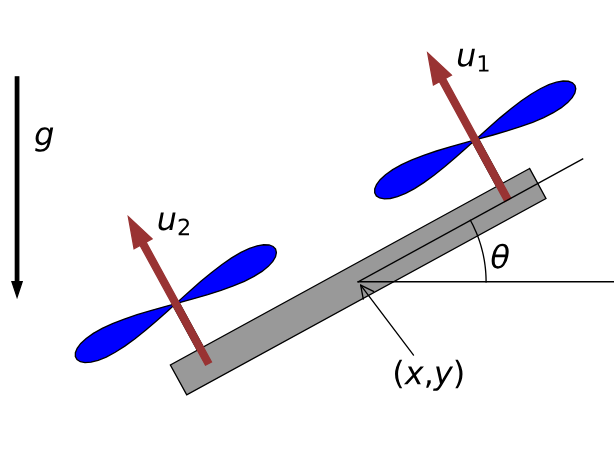
\includegraphics[width=0.3\textwidth]{quadrotor.png}
    \end{center}
\end{problem}

\begin{answer}
    The state vector $q$ can be defined as:
	\begin{align*}    
    \mathbf{q} = \begin{bmatrix} x \\ y \\ \theta \\ \dot{x} \\ \dot{y} \\ \dot{\theta} \end{bmatrix}
    \end{align*}
    The state space representation $\dot{q}$ can thus be defined as:
    \begin{align*}   
    \mathbf{\dot{q}} = \begin{bmatrix} \dot{x} \\ \dot{y} \\ \dot{\theta} \\ \ddot{x} \\ \ddot{y} \\ \ddot{\theta} \end{bmatrix}
    \end{align*}
    Based on the given dynamics, we can deduce that:
    \begin{align*}
        \ddot{x} &= {\frac{(- (u_1+u_2) \sin{(\theta)})}{m}} \\
        \ddot{y} &= {\frac{((u_1+u_2)\cos{(\theta)}-mg)}{m}} \\
        \ddot{\theta} &= {\frac{r(u_1-u_2)}{m}}
    \end{align*}
    Therefore,$\dot{q}$ can be defined as:
    \begin{align*}   
    \mathbf{\dot{q}} = \begin{bmatrix} \dot{x} \\ \dot{y} \\ \dot{\theta} \\ {\frac{(- (u_1+u_2) \sin{(\theta)})}{m}} \\ {\frac{((u_1+u_2)\cos{(\theta)}-mg)}{m}} \\ {\frac{r(u_1-u_2)}{m}} \end{bmatrix}
    \end{align*}
\end{answer}

\begin{problem}[10]
    Consider the nonlinear system
    \begin{align*}
        \dot{x}_1 &= x_2 \\
        \dot{x}_2 & = -a \sin{(x_1)} - bx_2
    \end{align*}
    with $a,b>0$.
    Find all the equilibrium points of this system.
\end{problem}

\begin{answer}
    To find equilibrium points of the nonlinear system, $\dot{x_1}$ and $\dot{x_1}$ equals to 0.
    So:
    \begin{align*}
        \dot{x}_1 &= x_2 = 0 \\
        \dot{x}_2 & = -a \sin{(x_1)} - bx_2 = 0
    \end{align*}
    So $x_2=0$ => $\sin{(x_1)} = 0$ => $x_1=n \pi$ where $n = 1,2,...$
\end{answer}

\begin{problem}[15]
    Let $X$ be a compact subset of $\mathbb{R}^n$. Prove that a contraction mapping $P: X \rightarrow X$ is a uniformly continuous function.
\end{problem}

\begin{answer}
    P is contraction mapping on X, therefore:
    \begin{align*}
    		d(P(x),P(y))<kd(x,y)(k \in [0,1))
    \end{align*}
    There exists a $\epsilon$ such that:
    \begin{align*}
    		d(x,y)<\epsilon
    \end{align*}
    There exists a $\delta$ such that:
    \begin{align*}
    		\delta &= \frac{\epsilon}{k}
    \end{align*}
    As such, we have:
    \begin{align*}
    		d(P(x),P(y))<\delta
    		d(x,y)<\epsilon
    \end{align*}
    Therefore, P is a uniformly continuous function.
\end{answer}

\begin{problem}[15]
    Consider the map
    \begin{align*}
        T(x) = rx(1-x)
    \end{align*}
    where $x \in \mathbb{R}$ (this is known as the "logistic" map). Define a set $U=[0,1]$. For what value of $r$ is this function $T$ a contraction map from $U$ to $U$?
\end{problem}

\begin{answer}
    To find r, we have to find derivative of T(x)
    \begin{align*}
    		T'(x)=r(1-2x)    		
    \end{align*}
    Since $U= [0,1]$:
    \begin{align*}
    		T'(0)=r
    		T'(-1)=-r
    \end{align*}
    Since T' is a linear function, max|T'(x)| = r
    For T to be a contraction map:
    \begin{align*}
    max|T'(x)| = r<1
    \end{align*}
    Therefore, r<1 so that T is a contraction map.
\end{answer}

\begin{problem}[15]
    Show that if $f_1: R \rightarrow R$ and $f_2: R \rightarrow R$ are locally Lipschitz, then $f_1+f_2$, $f_1f_2$ and $f_1 \circ f_2$ are locally Lipschitz. $\circ$ denotes function composition.
\end{problem}

\begin{answer}
    If  $f_1$ is locally Lipschitz, then:
    \begin{align*}
        |f_1(x_1)-f_1(x_2)|\leq k_1|x_1-x_2| (1)
    \end{align*}
    If  $f_2$ is locally Lipschitz, then:
    \begin{align*}
        |f_2(x_1)-f_2(x_2)|\leq k_2|x_1-x_2|(2)
    \end{align*}
    Then with (1) and (2), we have:
    \begin{align*}
    		f_1+f_2\\
        =>|[f_1(x_1)+f_2(x_1)]-[f_1(x_2)+f_2(x_2)]| \\
        \leq|f_1(x_1)-f_1(x_2)|+|f_2(x_1)-f_2(x_2)|\\
        \leq (k_1+k_2)|x_1-x_2|
    \end{align*}
    So $f_1+f_2$ is locally Lipschitz
    \begin{align*}
    		f_1f_2\\
        =>|f_1(x_1)f_2(x_1)-f_1(x_2)f_2(x_2)]| \\
        = |f_1(x_1)f_2(x_1)-f_1(x_1)f_2(x_2)+f_1(x_1)f_2(x_2)-f_1(x_2)f_2(x_2) |\\
        =|f_1(x_1)(f_2(x_1)-f_2(x_2))+f_2(x_2)(f_1(x_1)-f_1(x_2))|\\ 
        \leq |f_1(x_1)k_1+f_2(x_2)k_2||x_1-x_2|
    \end{align*}
    Let $L_1=sup_{x \in B(x_0,r)}|f_1(x_1)| $ and $L_2=sup_{x \in B(x_0,r)}|f_2(x_2)| $. The inequality above turns to:
    \begin{align*}
    		|f_1(x_1)(f_2(x_1)-f_2(x_2))+f_2(x_2)(f_1(x_1)-f_1(x_2))|\\ 
        \leq |L_1k_1+L_2k_2||x_1-x_2|
    \end{align*}
    So $f_1f_2$ is locally Lipschitz
    \begin{align*}
    f_1 \circ f_2\\
    => |f_1(f_2(x_1)) - f_1(f_2(x_2))| \leq k_1|f_2(x_1)-f_2(x_2)|\\
    \leq k_1k_2|x_1-x_2|
    \end{align*}
    So $f_1 \circ f_2$ is locally Lipschitz
\end{answer}

\begin{problem}[15] \cite{khalil2002nonlinear}
    Derive the sensitivity equations (in Python/MATLAB) with symbolic computation for the system
    \begin{align*}
        \dot{x}_1 &= \tan^{-1}(ax_1) -x_1x_2 \\
        \dot{x}_2 &= bx_1^2 -cx_2
    \end{align*}
    as the parameters $a,b,c$ vary from their nominal values $a_0=1, b_0=0$, and $c_0=1$.
\end{problem}

\begin{answer}
    \begin{lstlisting}
    % Define symbolic variables
syms x1 x2 a b c

% Define the system of equations
f1 = atan(a * x1) - x1 * x2;
f2 = b * x1^2 - c * x2;
M = [f1,f2];
lambda = [a,b,c];
x = [x1,x2];
A = jacobian([f1;f2],x);
B = jacobian([f1;f2],lambda)

    \end{lstlisting}
    We can denote $\lambda_0 =(a_0,b_0,c_0)=(1,0,1)$. Therefore, the sensitivity equation can be derived as:
    \begin{align*}
    		dot{S(t)}=[\begin{matrix}
    		a/(x_1^2 + 1) - x_2 & -x_1\\
    		0&-1
    		\end{matrix}]S(t)+
    		[\begin{matrix}
    		\frac{x_1}{x_1^2+1} & 0 & 0 \\
    		0 & x_1^2 & x_2^2
    		\end{matrix}] \\
    		S(t_0) = 0
    \end{align*}
\end{answer}

\begin{problem}[20]
    Consider the ordinary differential equation (ODE)
    \begin{align*}
        \frac{dx}{dt}=f(t,x), x(t_0) = x_0,
    \end{align*}
    where $f:\mathbb{R}\times \mathbb{R}^n\rightarrow\mathbb{R}^n$ is bounded and satisfies global Lipschitz condition on an interval $[t_0,t_1]$. Recall that the solution of this ODE can be written in the form as
    \begin{align*}
        x(t) = x_0 + \int_{t_0}^{t} f(s,x(s)) ds,\, \forall t\in[t_0,t_1]
    \end{align*}
    which is essentially the unique fixed-point of the contraction mapping $P[x](t) = x_0 + \int_{t_0}^{t} f(s,x(s)) ds$ defined on the Banach space $C^0([t_0,t_1])$. We also know that this fixed-point can be obtained iteratively using $x_{n+1} = P[x_{n}]$ and letting $n\rightarrow \infty$ (that is, $x^* = \lim_{n\rightarrow\infty} x_n$.)
    
    Let f(t,x)=7tx with x(3)=5, and the solution to this ODE is $x(t)=5 e^{\frac{7}{2}(t^2-9)}$. Verify this solution by applying this contraction mapping iteratively and demonstrate its convergence (in Python/MATLAB) with a plot that showing the approximation error relative to the analytical solution gradually decreases.

    HINT: $\sum_{k=0}^{\infty} \frac{x^k}{k!} = e^x$
    \end{problem}
\begin{answer}
    \begin{lstlisting}
t0 = 3;
t1 = 5;
x0 = 5; 
N = 100; 
max_iter = 10; 
t = linspace(t0, t1, N);
x_exact = @(t) x0 * exp((7/2) * (t.^2 - t0^2));
x_prev = x0 * ones(1, N);
errors = zeros(max_iter, 1);
for iter = 1:max_iter
    x_next = x0 + arrayfun(@(tt) integral(@(s) 7.*s.*interp1(t, x_prev, s, 'linear'), t0, tt), t);
    error = abs(x_next - x_exact(t));
    errors(iter) = max(error); % Store the maximum error
    x_prev = x_next;
end

figure;
plot(1:max_iter, errors, '-o');
xlabel('Iteration Number');
ylabel('Maximum Approximation Error');
title('Convergence of Fixed-Point Iteration');
grid on;
    \end{lstlisting}
    \begin{center}
        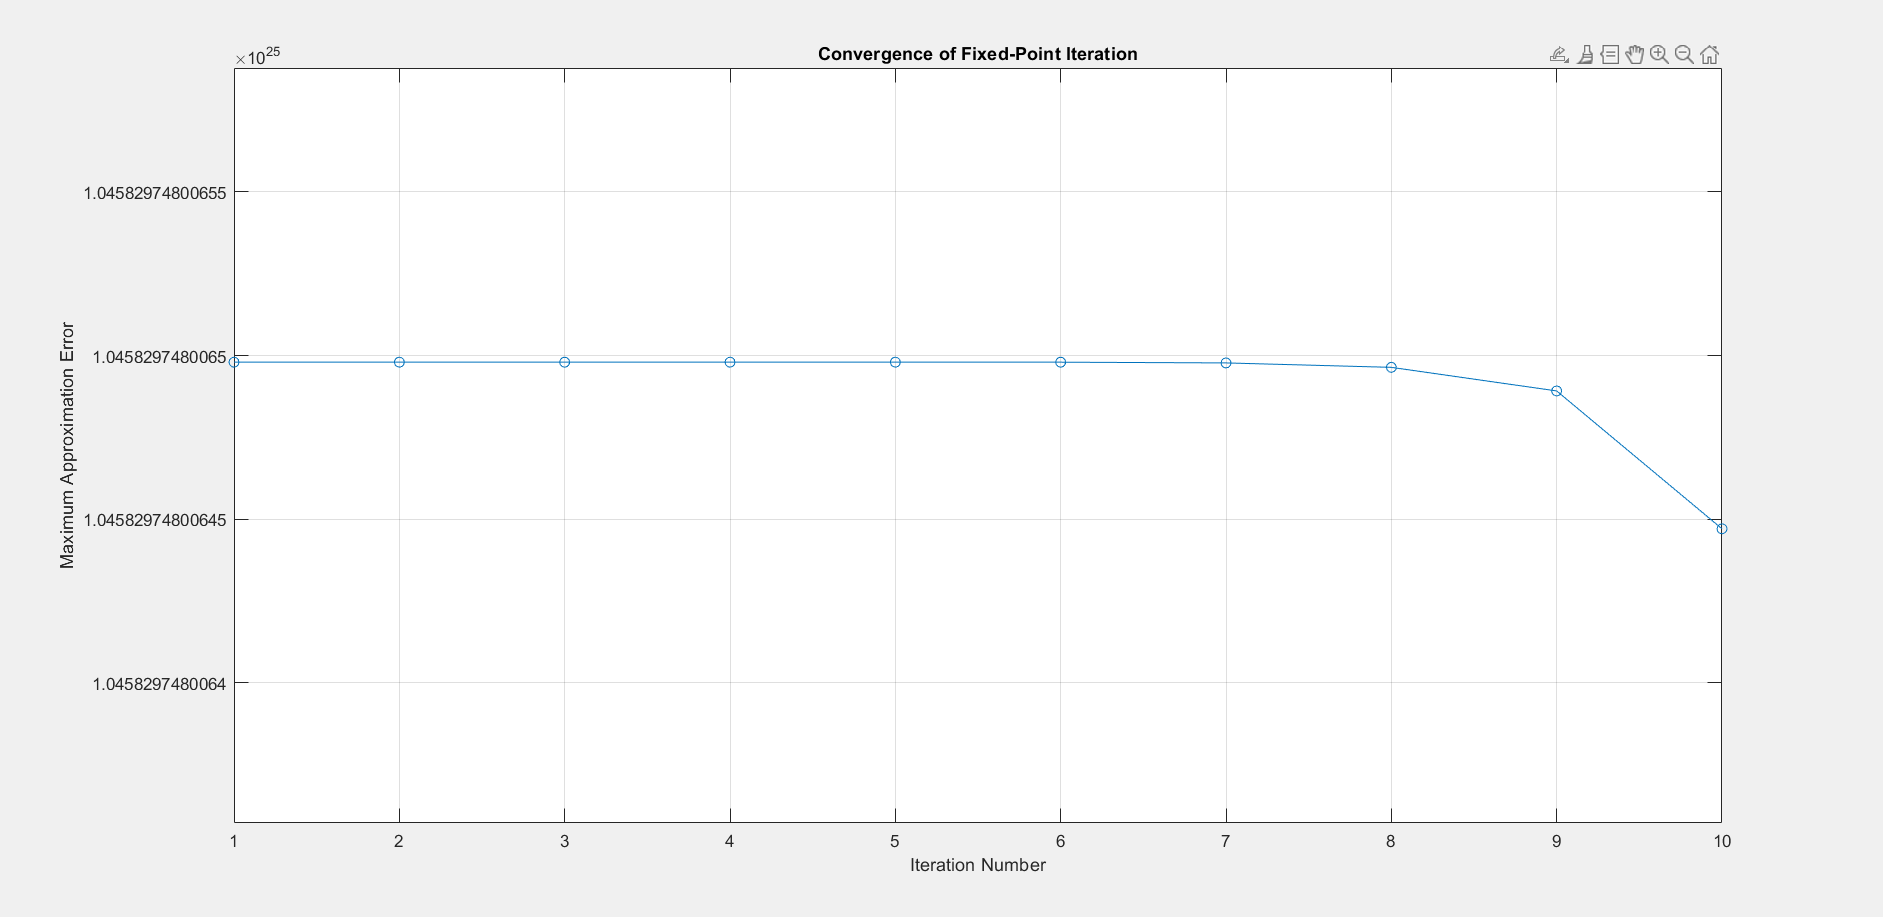
\includegraphics[width=0.9\textwidth]{esterr.png}
    \end{center}
\end{answer}



%------------------------------------------------
\bibliography{references}
\bibliographystyle{plainnat}

\end{document}